\documentclass[11pt]{article}
\usepackage[english]{babel}
\usepackage{geometry}
\usepackage{amsmath}
\usepackage{amsthm}
\usepackage{graphicx}
\usepackage[utf8]{inputenc}

%%%%%%%% MARGIN
\geometry{verbose, letterpaper, tmargin=3cm,
  bmargin=3cm,lmargin=2.5cm,rmargin=2.5cm}

%%%%%%%% PARAGRAPH SETTINGS
% https://tex.stackexchange.com/questions/27802/set-noindent-for-entire-file
\setlength\parindent{0pt}

% https://tex.stackexchange.com/questions/49188/how-to-insert-vertical-space-between-paragraphs
\setlength{\parskip}{5pt}

%%%%%%%% SUB-FIGURE PACKAGE
\usepackage{subcaption}

%%%%%%%% HYPERREF PACKAGE
\usepackage{hyperref}
\hypersetup{linkcolor=blue}
\hypersetup{citecolor=blue}
\hypersetup{urlcolor=blue}
\hypersetup{colorlinks=true}

%%%%%%%% DEFINITION AND THEOREM DEFINITIONS
\theoremstyle{definition}
\newtheorem{definition}{Definition}[section]

\theoremstyle{remark}
\newtheorem{remark}{Remark}

\theoremstyle{remark}
\newtheorem{question}{Question}

\newtheorem{theorem}{Theorem}[section]

%%%%%%%% MULTI-COLUMNS PACKAGE
\usepackage{multicol}

%%%%%%%% PERSONAL COMMANDS
\usepackage{amssymb}

%%%% Important sets
\renewcommand{\O}{\mathbb{O}}
\newcommand{\N}{\mathbb{N}}
\newcommand{\Z}{{\mathbb{Z}}}
\newcommand{\Q}{{\mathbb{Q}}}
\newcommand{\R}{{\mathbb{R}}}

%%%% Usual operations
\newcommand{\pow}[2]{#1^{#2}}
\newcommand{\expp}[1]{e^{#1}}
\newcommand{\fst}{\mathrm{fst}}
\newcommand{\snd}{\mathrm{snd}}

%%%% Lambda Calculus
\newcommand{\dneq}{\,\, \# \,\,}
\renewcommand{\S}{\pmb{\mathrm{S}}}
\newcommand{\I}{\pmb{\mathrm{I}}}
\newcommand{\K}{\pmb{\mathrm{K}}}
\newcommand{\ch}[1]{\ulcorner #1 \urcorner}

%%%% Ordinal Lambda Calculus
\newcommand{\ordAlph}{\Sigma_{\text{Ord}}}
\newcommand{\termOrd}{\text{Term}_\text{Ord}}
\newcommand{\fl}{\mathrm{fl}}
\newcommand{\sk}{\mathrm{sk}}

%% Superscript to the left
% https://latex.org/forum/viewtopic.php?t=455
\usepackage{tensor}
\newcommand{\app}[3]{\tensor*[^{#1}]{\left(#2, #3\right)}{}}

%%%% Make optional parameter
% https://tex.stackexchange.com/questions/217757/special-behavior-if-optional-argument-is-not-passed
\usepackage{xparse}

%%%% Statistics
\NewDocumentCommand{\E}{o m}{
  \IfNoValueTF{#1}
  {\mathbb{E}\left[#2\right]}
  {\mathbb{E}^{#1}\left[ #2\right]}
}
\NewDocumentCommand{\V}{o m}{
  \IfNoValueTF{#1}
  {\mathrm{Var}\left[#2\right]}
  {\mathrm{Var}^{#1}\left[ #2\right]}
}
\RenewDocumentCommand{\P}{o o m}{
  \IfNoValueTF{#1}
  {\IfNoValueTF{#2}
    {\mathrm{P}\left(#3\right)}
    {\mathrm{P}^{#2}\left(#3\right)}}
  {\IfNoValueTF{#2}
    {\mathrm{P}_{#1}\left(#3\right)}
    {\mathrm{P}_{#1}^{#2} \left(#3\right)}}
}

%%%% Lambda Calculus
\NewDocumentCommand{\cx}{o}{
  \IfNoValueTF{#1}
  {\left[\quad\right]}
  {\left[\, #1 \,\right]}
}

%%%% Create absolute value function
% https://tex.stackexchange.com/questions/43008/absolute-value-symbols
\usepackage{mathtools}
\DeclarePairedDelimiter\abs{\lvert}{\rvert}%
\DeclarePairedDelimiter\norm{\lVert}{\rVert}%
\makeatletter
\let\oldabs\abs
\def\abs{\@ifstar{\oldabs}{\oldabs*}}
%
\let\oldnorm\norm
\def\norm{\@ifstar{\oldnorm}{\oldnorm*}}
\makeatother

%%%%%%%% LOGIC TREES
\usepackage{prftree}

%%%%%%%% SPLIT EQUATIONS
% https://tex.stackexchange.com/questions/51682/is-it-possible-to-pagebreak-aligned-equations
\allowdisplaybreaks

%%%%%%%% FLOAT SPECIFIER
% https://www.overleaf.com/learn/latex/Errors/LaTeX_Error:_Unknown_float_option_%60H%27
\usepackage{float}

%%%%%%%% TO USE SHORT COMMANDS FOR VECTOR LINES
\usepackage{esvect}

%%%%%%%% ENUMERATE LABEL
% https://www.latex-tutorial.com/tutorials/lists/
\usepackage{enumitem}

%%%%%%%% DIFFERENT FONTS FOR MATH
\usepackage{mathrsfs}

%%%%%%%% CODE RENDERING !!! UNCOMMENT IF NEEDED !!!
% Compile with flag -shell-escape
\usepackage{minted}
\usemintedstyle{vs}

\newcommand{\code}[2]{\inputminted[frame=lines, linenos, firstline=#1,
  lastline=#2]{cpp}{../src/roman-numerals.cpp}}

%%%%%%%% START DOCUMENT

\title{UVa: 185 - Roman Numerals Solution}
\author{Andrés Felipe Tamayo \\
  \scalebox{0.7}{aftamayoa@eafit.edu.co} \and
  Juan Sebasti\'an C\'ardenas-Rodríguez \\
  \scalebox{0.7}{jscardenar@eafit.edu.co}}

\date{\scalebox{0.7}{Mathematical Engineering, Universidad EAFIT} \\[2ex]
  \today}


\begin{document}
\maketitle

\section{General Remarks}
For the solution of this problem, three variables are obtained in the following
manner:
\begin{equation*}
  \mathtt{first}+\mathtt{second}=\mathtt{ans}
\end{equation*}

for which \texttt{second} is the biggest word between the left hand side of the
equation. It is important to remark that each problem was stored in an abstract
class called \texttt{Problem}, which solves each of the equations and outputs
the needed output. Variable assignation will be noted by $\equiv$.

Lastly, it was coded in \texttt{c++} and tested with the Ubuntu compiler
\texttt{g++ 7.5.0}. This code was also with tested with the debug data set given
in \href{https://www.udebug.com/UVa/185}{UVa debug} which passed all tests and
the \href{https://onlinejudge.org/}{online judge} which ran with a time of
0.000ms and ranks as the 43th best solution to date.

\section{Roman Sum}

\subsection{Data Structures}
Each of the three variables are stored as a data type \texttt{string}.

\subsection{Algorithm}
The algorithm that find if the equation is a correct roman sum, first needs an
procedure that transform a given \texttt{string} variable to the respective
roman integer number.
%
\begin{table}
  \centering
  \begin{tabular}{cccc}
  \hline
  I   &   $1$ & V &$5$ \\
  X   &  $10$  & L & $50$ \\
  C   & $100$ & D &  $500$  \\
  M  & $1000$  & \\
  \hline
  \end{tabular}
  \caption{Roman characters to decimal representation.}
  \label{tab:romChar}
\end{table}
%
In the first place, a function that transforms a given roman character to their
respective integer value is given in Table \ref{tab:romChar}. Then, to transform
a roman numeral it's decimal number representation the following procedure is
executed:
%
\begin{enumerate}
  \item Initialize two variables, \texttt{num} which will have accumulate each
    of the respective digits and \texttt{lastChar} which will save the last
    character that was evaluated. Both of them are initialized at the value of
    the first character.
  \item The next character of the string is converted to a number.
  \item If the last character has a smallest value that the actual character
    evaluated, \texttt{num} is updated in the following manner:
    %
    \begin{equation*}
      \mathtt{num} \equiv \mathtt{num} - 2*\mathtt{lastChar}
    \end{equation*}
    %
  \item The value of the actual character is summed to \texttt{num}. Continue
    repeating from step 2 till all characters of the string are used.
\end{enumerate}
%
The algorithm for this process is given by: \code{105}{116}
%
Therefore, to find if the equation is a correct roman numeral sum both
\texttt{first} and \texttt{ans} are transformed to their decimal representation.
If \texttt{first} is bigger than \texttt{ans}, then it is automatically flagged
as an incorrect solution. If not, then \texttt{second} is transformed to its
decimal representation and the sum is checked as needed by the problem.

\section{Arabic Sum}

\subsection{Data Structures}
There are mainly two data structures used to represent the roman numeral as
their Arabic counterpart. In the first place, there is an \texttt{vector} that
stores the value for each of the letters named \texttt{list}. Lastly, there is
an \texttt{array} of size 7 that stores in which index of the previous structure
is the letter stored named \texttt{indexes}. A representation of this array can
be seen in Figure \ref{fig:indRep}.

\begin{figure}[H]
  \centering
  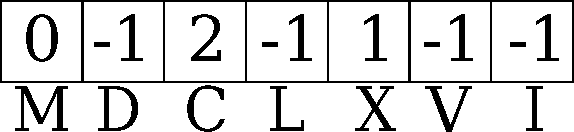
\includegraphics[scale=.5]{figs/index-roman}
  \caption{Index representation of letters.}
  \label{fig:indRep}
\end{figure}

To initialize this arrays, the first step is to define ranges for each of the
letters in order to restrict the domain of the value for each letter. To create
the ranges for a character there are some special cases. To see examples for the
two special cases see the following:

\begin{multicols}{2}
  \noindent
  \begin{table}[H]
    \centering
    \begin{tabular}{ccc}
      & V & I \\
    + & I & I \\ \hline
    X & L & V
    \end{tabular}
  \end{table}
  In this case, it is clear that $\text{X}=1$. This occurs when the length of
  \texttt{ans} is bigger than the length of \texttt{second}.
  %
  \columnbreak
  %
  \begin{table}[H]
    \centering
    \begin{tabular}{ccc}
      &   & I \\
    + & M & I \\ \hline
    X & L & V
    \end{tabular}
  \end{table}
  In this case, it is clear that, in addition to the previous case, $\text{M}=9$
  and $\text{L}=0$. This occurs when it is also satisfied that the length of
  \texttt{first} is smaller than the length of \texttt{second}.
\end{multicols}

\begin{enumerate}
  \item If the character satisfies one of the special cases, a fixed range is
    selected of the form $[\delta, \delta]$, where $\delta$ is a fixed integer
    given by the special case.
  \item Otherwise, if the character is an initial character of a string then the
    ranges is given by $[1, 9]$ otherwise it is given by $[0, 9]$.
\end{enumerate}

Following this procedure, each of the ranges is saved in a \texttt{vector} that
stores each of the ranges for the letters called \texttt{ranges}. Furthermore,
in the array \texttt{indexes} the position of the range of the respective letter
in \texttt{ranges} is stored. The functions that realize this operations are
given by \texttt{obtainRanges} and \texttt{filLRanges}.

After the ranges are created, then the initial value for each of the respective
letters are selected by the following procedure:
\begin{itemize}
  \item In the first place, the initial value for the letters that satisfied a
    special case are selected as $\delta$ and saved in \texttt{list} in the same
    index as the respective range. If another letter already has this value,
    then there isn't a solution.
  \item Lastly, each of the elements of the vector \texttt{list} is initialized
    by the first value of its range that is not used. In case that a letter does
    not have a possible not used number, there is not a solution.
\end{itemize}

The algorithm for this procedure is given by: \code{145}{175}

In conclusion, at the end of all this initialization the class \texttt{Problem}
ends with three data structures. The array \texttt{indexes} which has a -1 in
the letters that do not appear on the equation and a positive or null value
representing the index in the vector. A vector \texttt{ranges} which saves the
respective ranges of all the letters, in the respective indexes. And lastly, a
vector \texttt{list} which contains the initial testing values for each of the
letters.

\subsection{Solution Space}
As each of the letters is signified by a position in a list, then the solution
space for the problem is given by a point in a discrete coordinate. Therefore,
if $n$ is the number of unique characters between all the three variables then
the solution space is given in
%
\begin{equation*}
  \mathrm{SS} = \Lambda^{n}, \text{ where } \Lambda = \{0,1,2,\ldots,10\}
\end{equation*}
%
where $\Lambda^{n} = \underbrace{\Lambda \times \ldots \times \Lambda}_{n \text{
    times}}$, where $\times$ is the cross product.

Therefore, if the problem was solved by a brute force approach, the worst case
scenario is when there is not a possible solution for the arabic sum. Therefore,
all the possible permutations have to be evaluated. Furthermore, this worst case
scenario also includes that none of the special cases are satisfied. Therefore,
the number of evaluations is given by:
%
\begin{equation*}
  \mathrm{NE} =
  \begin{cases}
    \mathrm{P}(9, 3), &n = 3 \\
    \mathrm{P}(9, 3) \cdot \mathrm{P}(7, n - 3), &n > 3
  \end{cases}
\end{equation*}

where $\mathrm{P}(\cdot, \cdot)$ is the permutation function.

\subsection{Backtracking Strategy}
For the backtracking strategy the idea is to discard elements in the solution
space such that the sum of the last characters for \texttt{first} and
\texttt{second} (module 10) is not equal to the last character of \texttt{ans}.
In this manner, this are examples of discarded and non discarded solutions:
%
\begin{itemize}
  \item Discard: $V3 + X4 = L5$
  \item Discard: $V8 + X4 = L3$
  \item Approved: $V3 + X4 = L7$
  \item Approved $V6 + X7 = L3$
\end{itemize}
%
This allows only find list combinations that satisfy the respective sum and,
therefore bounds the space of the solution. The algorithm that discards this
solutions till it satisfies the required restriction is done by the following:
\code{315}{338}

\subsection{Algorithm}
Therefore, to find the desired output the algorithm just backtracks according to
the strategy explained above and tests for valid solutions. If backtracking is
not necessary, next combinations for the list are generated. The algorithm that
executes this is done by the following: \code{342}{362}

One other important detail is the algorithm that finds the next combination for
which the space solution is going to be evaluated. This algorithm does the
following:
\begin{enumerate}
  \item It starts checking the last index of the list.
  \item The value of that index is increased by one (module the largest possible
    value it can have) until it finds a non used number or it returns to the
    initial value for that item.
  \item If a non used number is found, that value is set for that index and the
    algorithm stops.
  \item If the value returns to their initial value, then it is set to -1 and
    the process repeats step 2 with the previous character. If no previous
    character exists, then there is no next combination.
  \item Lastly, all the -1 are replaced for the first value on their range that
    is not used.
\end{enumerate}

The algorithms that execute the previous procedure are given by: \code{246}{264}
\code{267}{281} \code{284}{288}

\end{document}
